\documentclass{roadef}
\usepackage{amsmath}
\usepackage{booktabs}

% \usepackage{fontspec}
% This command is to use simple quotes inside math expressions:
\newcommand{\mq}[1] {#1\textrm'}

\begin{document}


% Le titre du papier
\title{ROADEF Challenge 2018: Cutting Optimization Problem Description}

% Le titre court
% \def\shorttitle{Titre court}

\author{Franco Peschiera\inst{1}, Nicolas Dupin\inst{2}, Luca Mossina\inst{1}}


\institute{
ISAE-SUPAERO, Université de Toulouse, France \\
Laboratoire de recherche en informatique, Université de Paris-Sud \\
\email{\{franco.peschiera,luca.mossina\}@isae-supaero.fr,dupin@lri.fr}
}


\maketitle
\thispagestyle{empty}

\section{Introduction}

This report presents an algorithm for solving the cutting optimization problem of the Roadef 2018 challenge.
The problem consists in deciding how to cut a sequence of same-size jumbos in order to obtain all necesary items according to a sequence and required sizes taking into account jumbos' defects and cutting limits.

Our approach is based on the combination of two different metaheuristics—namely simulated annealing
and variable neighborhood search (VNS). 


\section{Solution coding}

        The solution is stored as a forest, where each jumbo is represented by a tree and each cut produces new children nodes. If a node is not a leaf, then it has been cut. Its children represent the number of cuts it has received, following the rules of guillotine cuts.
        Each children node has a level that is 1 bigger than its parent, so the level determines the depth of the node in the tree.

        For example, the solution shown in figure \ref{fig:case1} is represented by the following tree:

        \begin{tiny}
        \begin{verbatim}

                      /-2
                     |
                   /1|--3
                  |  |
                  |  |   /-5
                  |   \4|
                  |      \-6
                  |
                  |   /-8
                  |-7|
                  |   \-9
                -0|
                  |   /-11
                  |  |
                  |  |   /-13
                  |-10-12
                  |  |   \-14
                  |  |
                  |   \-15
                  |
                   \-16

        \end{verbatim}
        \end{tiny}

        \begin{figure}
            \centering
            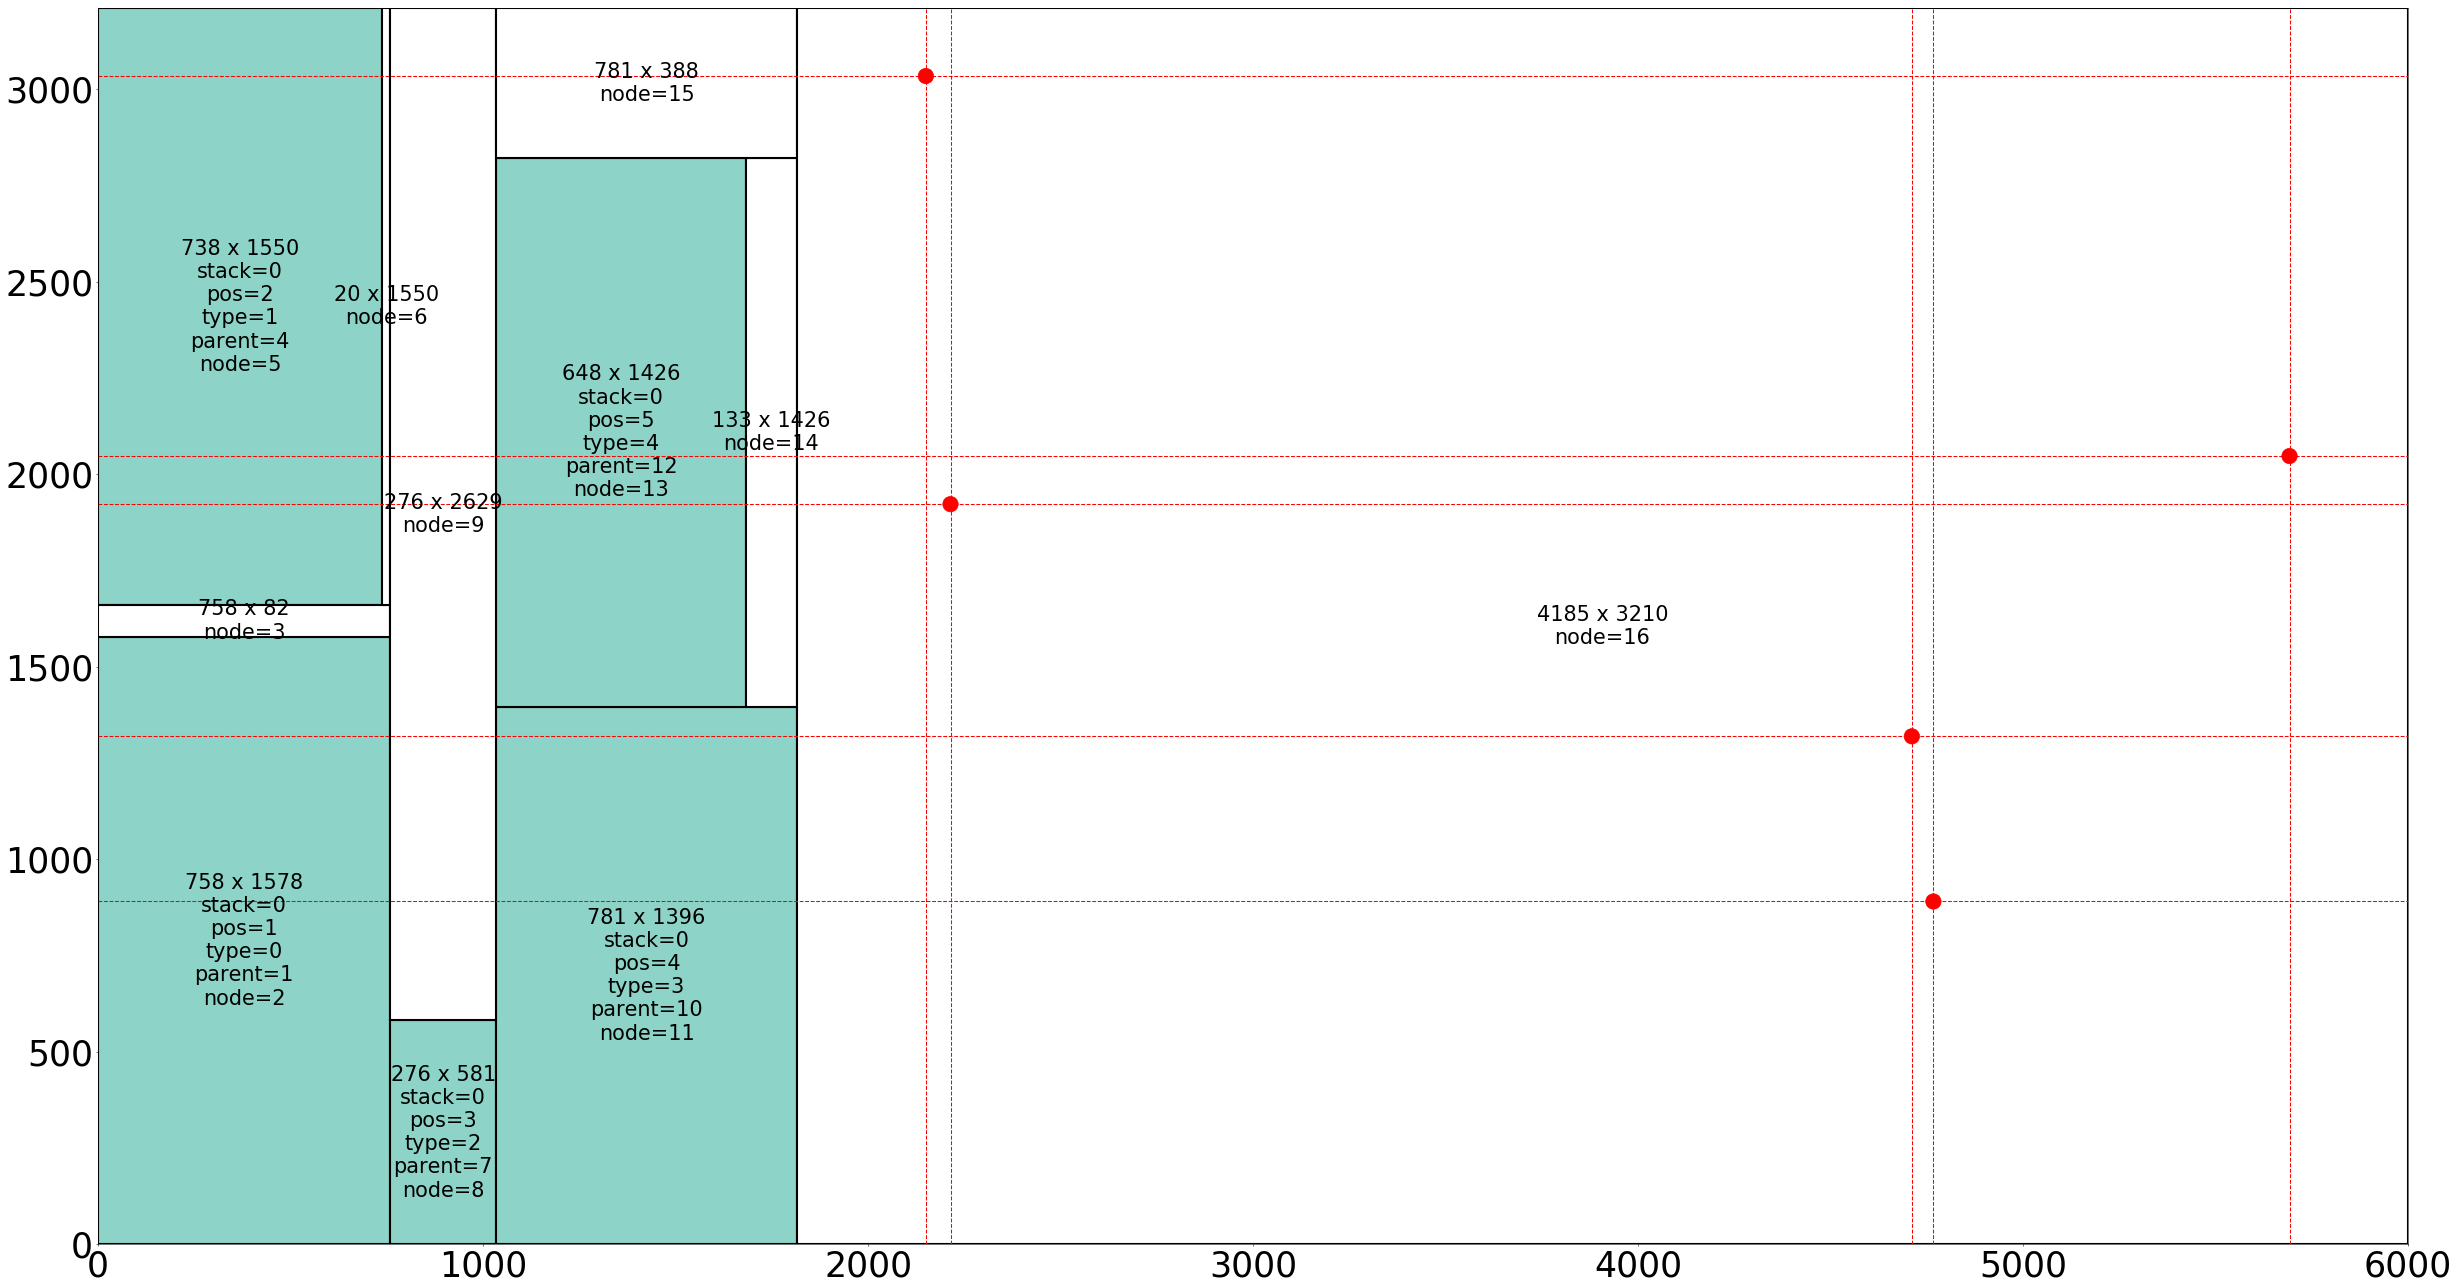
\includegraphics[width=0.4\linewidth]{case1_heur.png}
            \caption{case1 solution} \label{fig:case1}
        \end{figure}

        In addition to regular information related to its parent and children, a node also has information on its physical position: (PLATE, X and Y coordinates); its size (WIDTH and HEIGHT); type (waste, item code, intermediate node); and cut (the depth of the node in the tree).

\section{Allowed moves}

    Swaps are the main way to modify a solution. There are two main types of swaps: insertion or exchange. In the insertion, a node is extracted from its place and inserted before a given node, adapting the rest nodes accordingly. In the exchange, two nodes are extracted in positioned one instead of the other. For both of this functions, the extracted nodes can be rotated or not just before (re)insertion.

    The nodes to be swapped can be any type of node (a waste, an intermediate node or an item) and almost any level (the root node of a tree and nodes of level 4 nodes are exceptions).

    \subsection{Choosing candidates}

        Candidates can be obtained in several ways. Nodes that make the solution infeasible because of a sequence error or a defect are primary candidates. Also, waste nodes that are too close to the beginning of the solution and item nodes too close to the end.

    \subsection{Evaluating candidates}

        In order to make a feasible swap, it's necessary to check the following conditions: in an exchange, each node should be smaller than the space left by the other node plus the available sibling waste; in an insertion, the inserted node needs to be smaller than the available sibling waste the other node.

        If there is not enough space to do the swap, it is not done. The current solution complies with the borders and dimensions so no overlapping can exist between nodes.

        While checking for enough space, a simulation of the waste modification process is done. This way: all new positions are calculated for all relevant items in order to determine new defect violations after the swap.

        To evaluate the improvement of the swap we need to: 1. calculate the balance of sequence violations, 2. the balance of defect violations and 3. the balance of mean item density. Since we conceive a solution with sequence violations and defect violations, we measure the change in each of these values.

        We calculate the weighted sum of all three criteria. Weights are determine as a configuration and are not modified during the solving process.

        When comparing several candidates, we choose a random candidate, with a probability weighted by the quality of the swap. The selected candidate swap is then done according to a simulated annealing rule (so we accept worse solutions if high enough temperature).

    \subsection{Inserting a node somewhere}

        This is the basic logic to insert a node inside a destination node. This is use as the base for all the swaps mentioned above.

        \begin{enumerate}

            \item Take out children waste from each node. This is the waste that's at the end if any.
            \item If only child, take out and decrease level.
            \item If rotation is needed, rotate the whole node.
            \item Insert node in its destination parent.
            \item If the level of the node has changed, update it.
            \item if the node corresponds to actually several nodes, get them out and re-insert them.
            \item if needed, add a children waste on the node(s) that has /have just been inserted.
            \item Since a node has just been inserted, modify the residual waste at the end of the destination node.

        \end{enumerate}

    \subsection{Example swap}

        Figures \ref{fig:swap3-before} and \ref{fig:swap3-after} show an insert from a level 3 node (node 88, red) just before a level 2 (node 74, yellow) node while rotating it before insertion.

        \begin{figure}
            \centering
            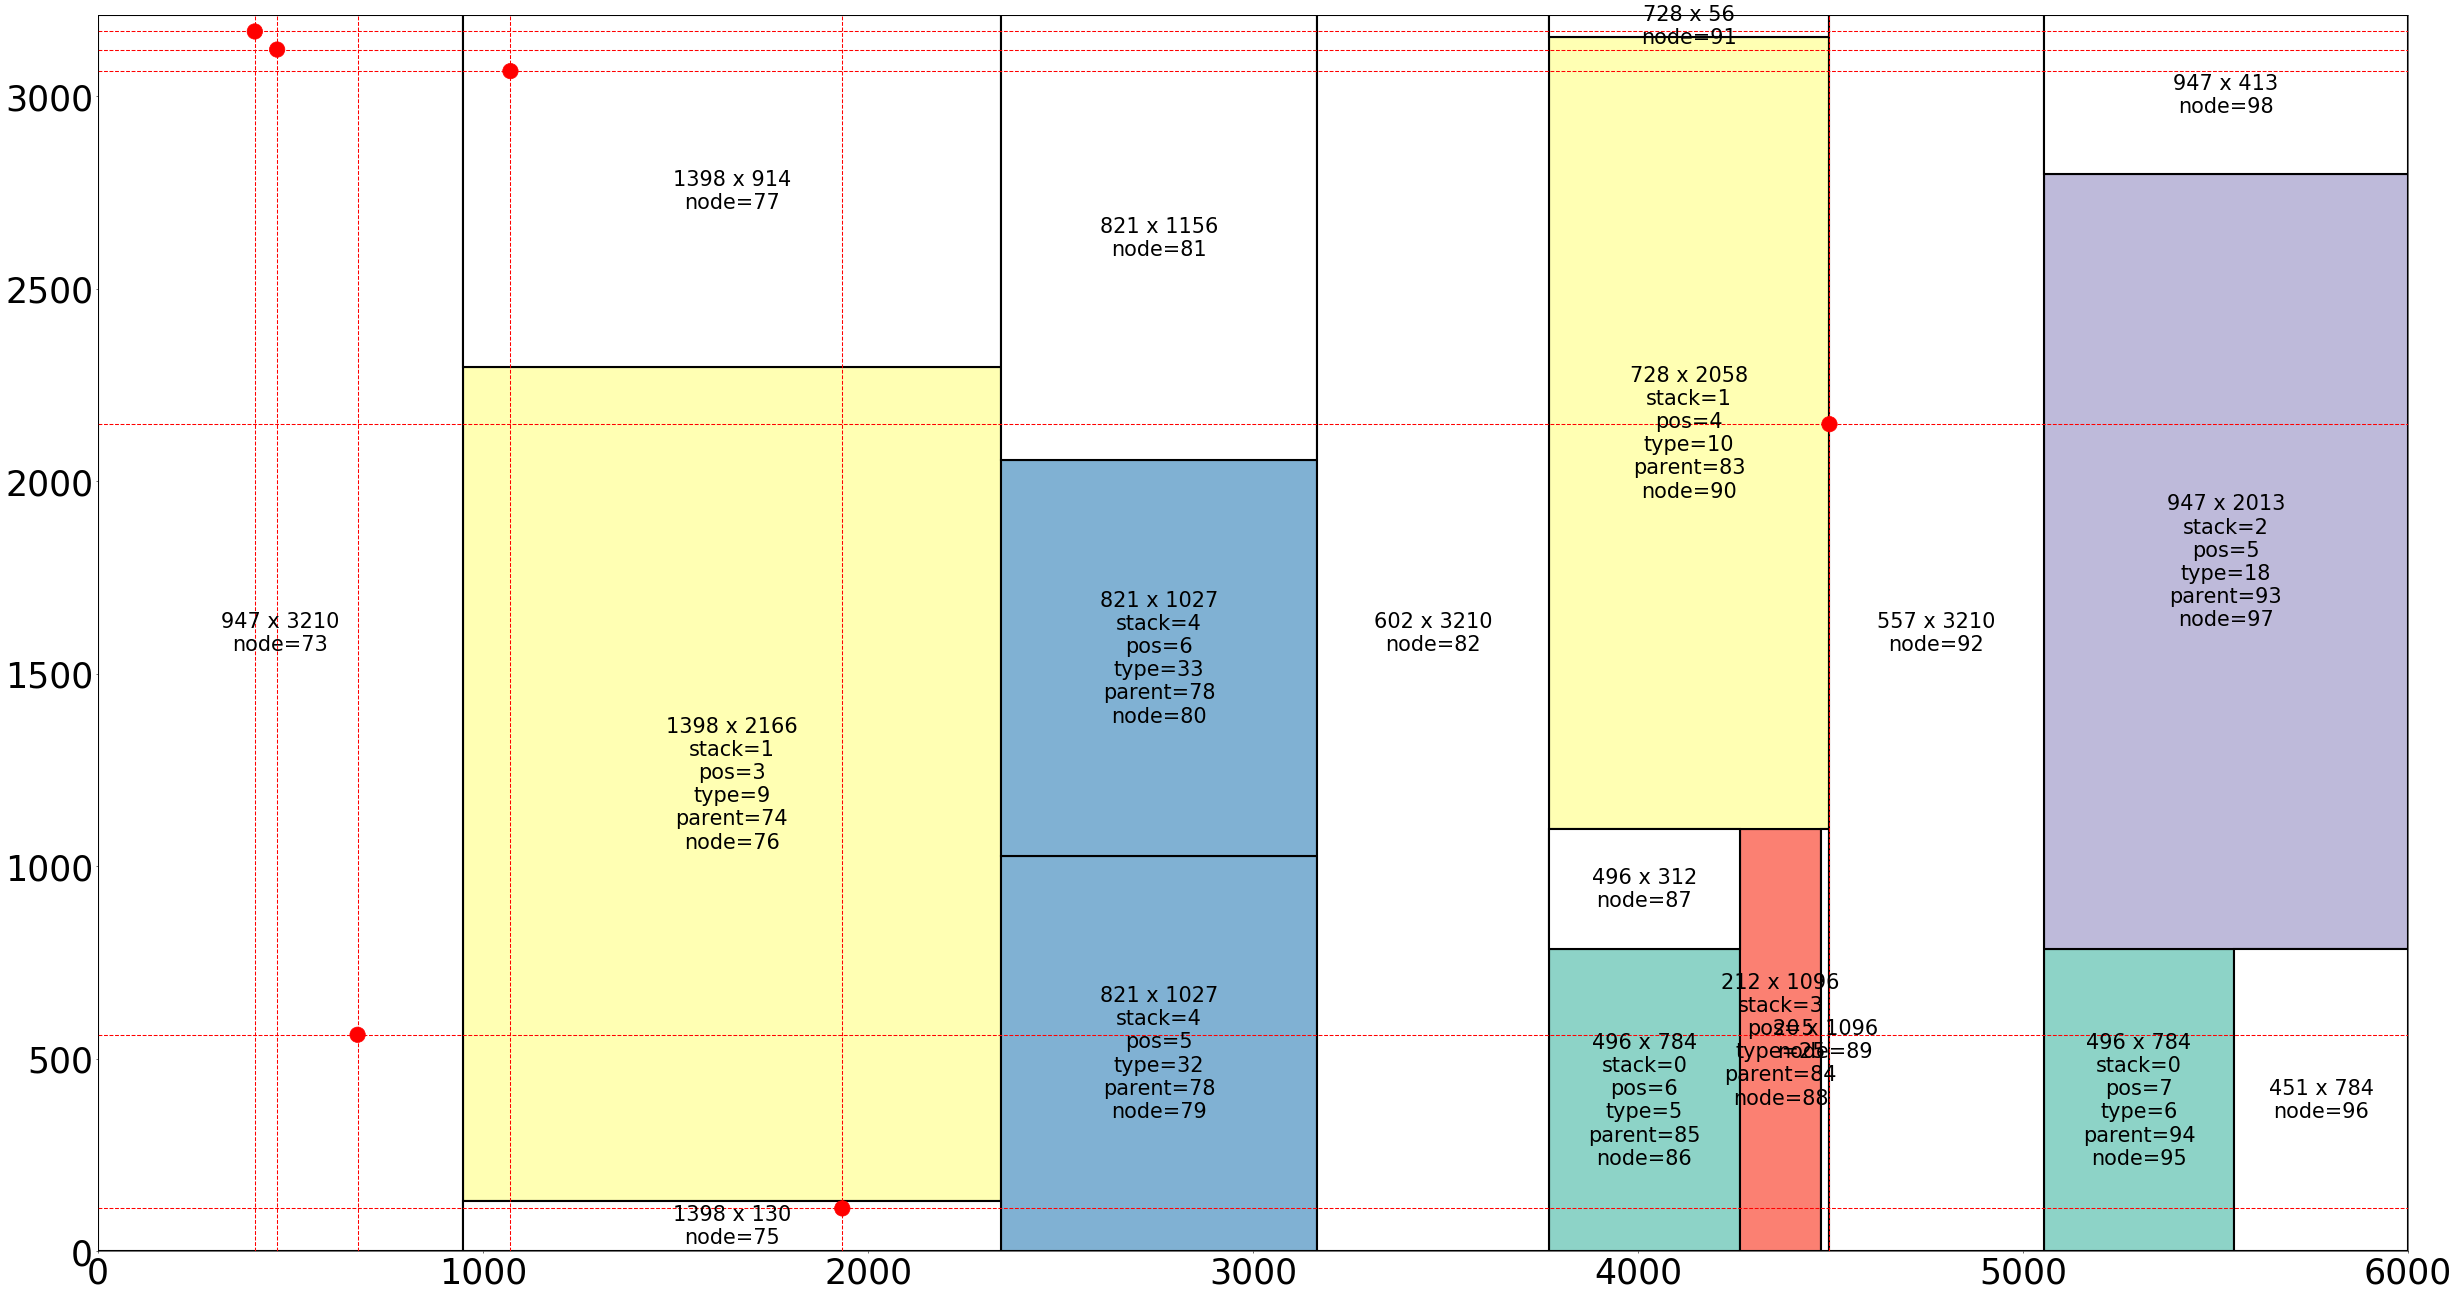
\includegraphics[width=0.4\linewidth]{swap_3_rot_before.png}
            \caption{before swap level 3} \label{fig:swap3-before}
        \end{figure}

        \begin{figure}
            \centering
            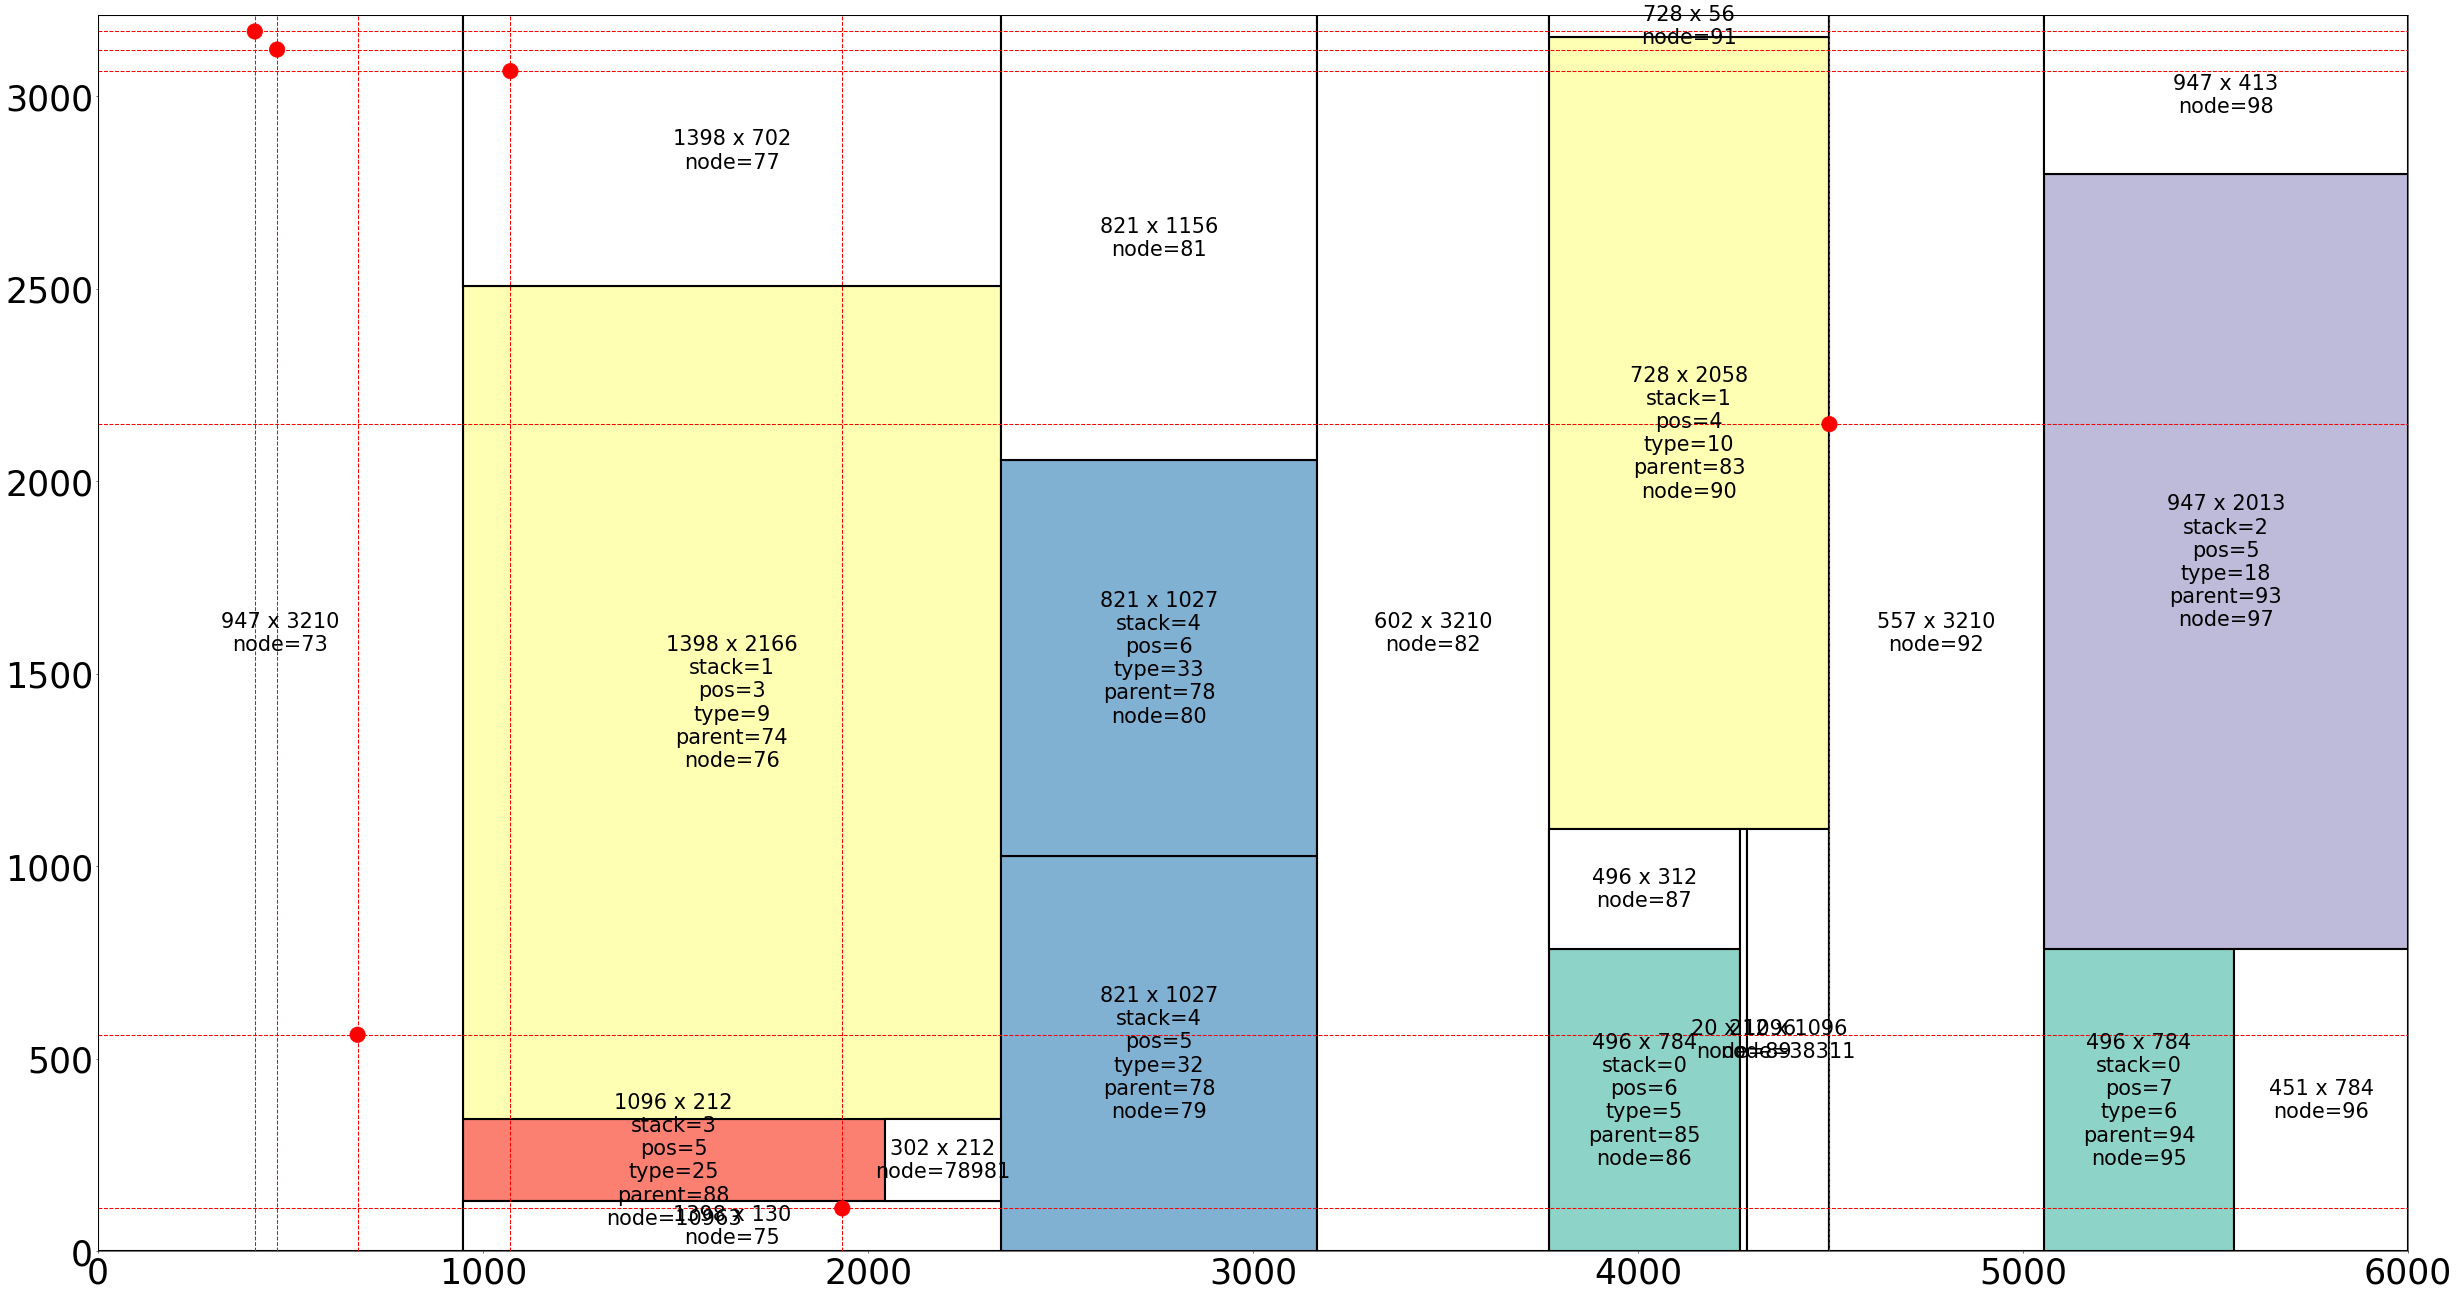
\includegraphics[width=0.4\linewidth]{swap_3_rot_after.png}
            \caption{After swap level 3} \label{fig:swap3-after}
        \end{figure}

\section{Optimization}

    \subsection{Construction algorithm}

        An initial solution is done by ordering the nodes with several (random) feasible sequences and trying to insert them one after the other in the first available feasible whole in the jumbos. The best solution of all simulated is kept as an initial solution.

        % This construction algorithm is used during the solving process to recreate parts of the current solution by reordering the items in a group of consecutive jumbos.

    \subsection{Simulated annealing}

        The following changes are done at any of the three levels (between nodes of level 1, nodes of level 2 and nodes of level 3).

        \begin{enumerate}

            \item try to merge wastes that are neighbours into one single waste.
            \item create waste cuts following the positions of defects
            \item push wastes to the right of the solution (to the end).
            \item do swapping in same level to correct sequence.
            \item do swapping in same level to correct defects.
            \item do swapping in the same level from random pairs of nodes.
            \item make inter-level swaps of 1 level difference (1 and 2, 2 and 3, 3 and 4).
            \item make inter-level swaps of 2 level difference (1 and 3, 2 and 4).
            \item if not many changes, remake solution by:

            \begin{enumerate}
                \item reordering a sequence of jumbos of size 1-4, 
                \item restarting to another initial solution,
                \item restarting to the best solution found.
            \end{enumerate}

        \end{enumerate}

    \subsection{Variable neighborhood search}

        A VNS algorithm was executed every X iterations of the main algorithm. This subroutine partially recreates the solution by generating several alternative consecutive jumbos to replace in the current solution. This is then tested to see if improves or not the quality of the solution and is accepted with a low probability if it decreases the objective function.

\section{Implementation}

    All the code is built in the python programming language (tested with versions 3.5 and 3.6). The code is available at the following repository: https://github.com/pchtsp/roadef2018. There, instructions on how to install it, deploy it and use it can be found, including a README file and a requirements file.

    Some modules were compiled using cython into C code for faster execution. Also, multiple processors where used in during the initial solution and the VNS algorithm to improve the execution time.

\section{Results}

The following results were obtained with a Fedora 62 GB RAM server with 12 cores and CPU speed (in MHz) of 2927.000.

\begin{tabular}{lr}
\toprule
instance &  objective \\
\midrule
      A1 &     425486 \\
      A3 &   11874210 \\
      A4 &   33153300 \\
      A5 &   18848943 \\
      A6 &   17709450 \\
      A7 &   19871010 \\
      A8 &   54429614 \\
      A9 &   12900966 \\
     A10 &   28255681 \\
     A11 &   30379189 \\
     A12 &    9099244 \\
     A13 &   72359643 \\
     A14 &   80907078 \\
     A15 &   87772601 \\
     A16 &   10435913 \\
     A17 &    6804781 \\
     A18 &   31129068 \\
\bottomrule
\end{tabular}


\bibliographystyle{plain}

\end{document}
